\documentclass{beamer}
%

% Choose how your presentation looks.
%
% For more themes, color themes and font themes, see:
% http://deic.uab.es/~iblanes/beamer_gallery/index_by_theme.html
%
\mode<presentation>
{
  \usetheme{NYU}      % or try Darmstadt, Madrid, Warsaw, ...
  \usecolortheme{default} % or try albatross, beaver, crane, ...
  \usefonttheme{default}  % or try serif, structurebold, ...
  \setbeamertemplate{navigation symbols}{}
  \setbeamertemplate{caption}[numbered]
} 

\usepackage[english]{babel}
\usepackage[T1]{fontenc}
\usepackage[utf8x]{inputenc}
\usepackage{hyperref}
\usepackage{graphicx}

\title[Assignment]{CONTROL SYSTEMS}
\subtitle{ASSIGNMENT 1}
\author{Adyasa Mohanty}
\institute{IIT HYDERABAD}
\date{\today}


\begin{document}

\begin{frame}
  \titlepage
\end{frame}

\begin{frame}{Question}
  \content {The impulse response of a system is h(t)= t u(t).For an input u(t-1), the output is:\\\vspace{15}A)  $\frac{t^2}{2}u(t)$ \enspace B) $\frac {t(t-1)}{2}u(t-1)$ \enspace C)$\frac{(t-1)^2}{2}u(t-1)$ \enspace D)$\frac{t^2-1}{2}u(t-1)$ }
\end{frame}
\begin{frame}{Solution}
  \content {\qquad Laplace Transform\\\vspace{5mm}
  $F(s)= \int_0^\infty f(t)\frac{1}{e^(st)}dt $\\\vspace{5mm}
  \qquad f(t) \qquad F(s)\\\vspace{5}
  \qquad 1    \qquad  $\frac{1}{s}$\\\vspace{5}
  \qquad $t$    \qquad  $\frac{1}{s^2}$\\\vspace{5}
  \qquad $u(t)$ \qquad  $\frac{1}{s}$\\\vspace{5}}
\end{frame}

\begin{frame}{Solution}
  \content {Impulse response of system is h(t)= tu(t)\\\vspace{5mm}Input x(t)=u(t-1)\\\vspace{5mm}The output will be y(t)= x(t)*h(t)\\\vspace{5mm}Taking Laplace transform on both the sides we get\\\vspace{5mm}$Y(s)=X(s)H(s)=\frac{1}{se^s}\times \frac{1}{s^2}=\frac{1}{s^3e^s}$\\\vspace{5mm}}
\end{frame}
\begin{frame}{Solution}
  \content {Taking the inverse Laplace Transform we get \\\vspace{10} \qquad $y(t)=p(t-1)$ \\\vspace{10}where p(t)= parabolic function\\\vspace {10} \qquad $\frac{1}{s^3}=\frac{t^2}{2}u(t)$\\\vspace{10} \qquad $\frac{1}{e^ss^3}=\frac{(t-1)^2}{2}u(t-1)$}
\end{frame}

\begin{frame}{Solution}


\centering
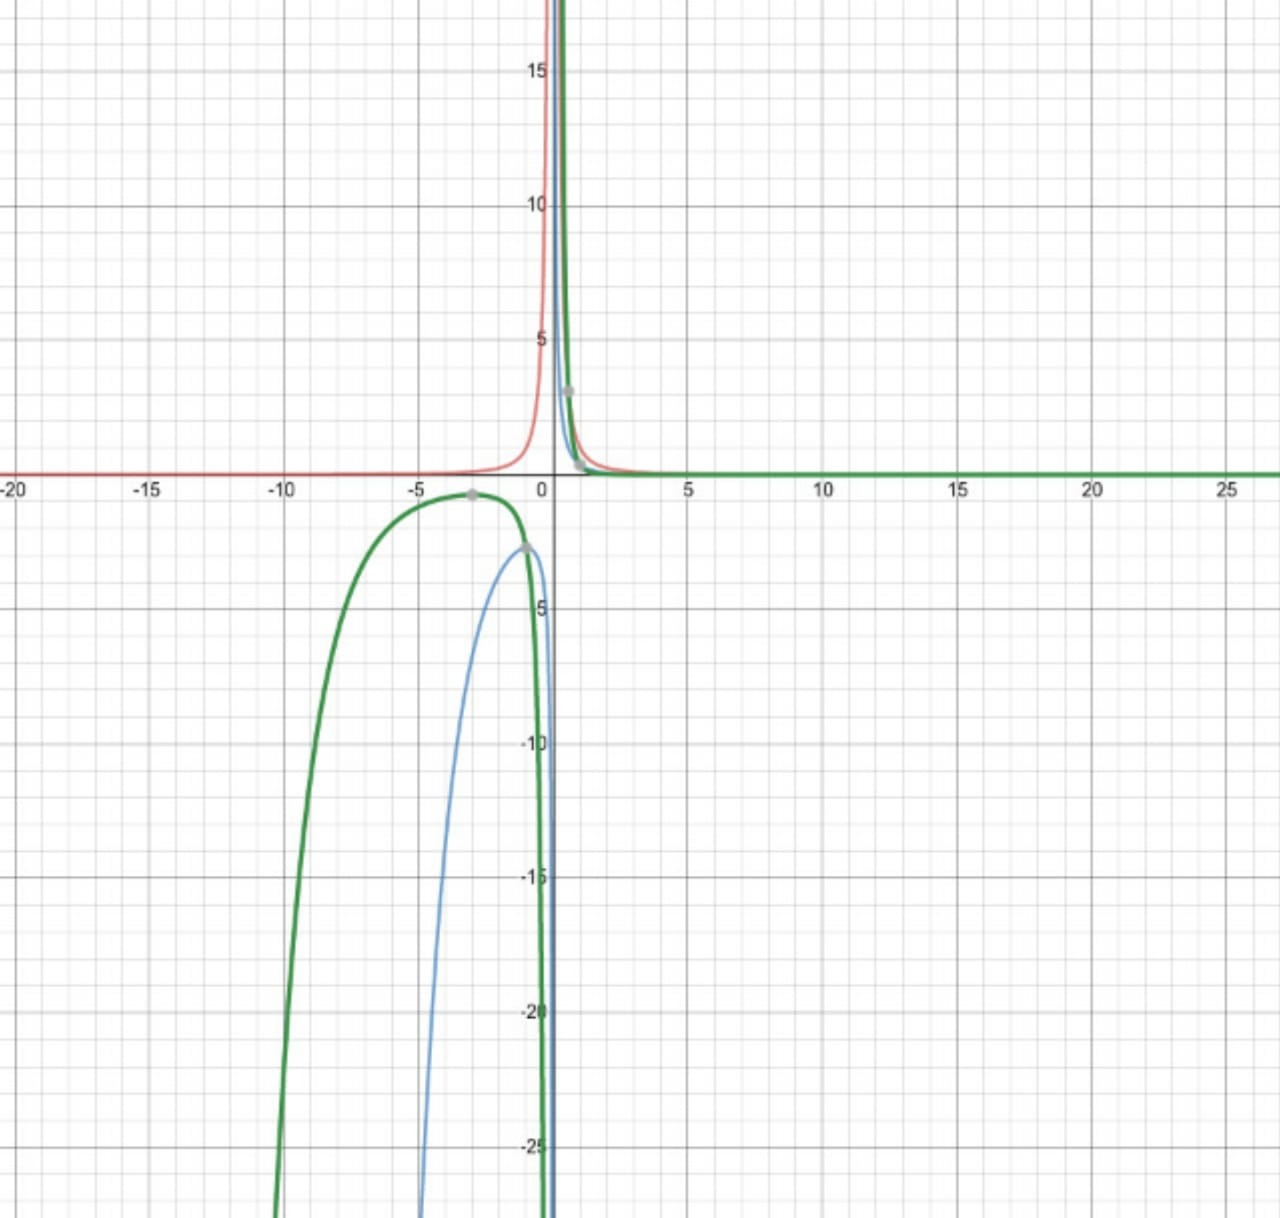
\includegraphics[width=6cm]{t.jpeg}
\end{frame}

\end{document}
